\documentclass[11pt]{article}
\usepackage[utf8]{inputenc}
\usepackage[T1]{fontenc}
\usepackage{lmodern}
\usepackage[margin=2.3cm]{geometry}
\usepackage{amsmath,amssymb}
\usepackage{graphicx}
\usepackage{url}
\renewcommand{\figurename}{Figura}
\renewcommand{\tablename}{Tabla}
\renewcommand{\refname}{Referencias}
\renewcommand{\abstractname}{Resumen}
\renewcommand{\contentsname}{Contenido}
\title{Reconstrucción y eliminación de ruido en imágenes con K-SVD:\\ una adaptación didáctica}
\author{Proyecto académico --- Matemáticas Computacionales, INAOE}
\date{}
\begin{document}
\maketitle
\begin{abstract}
Se implementa un ciclo K-SVD propio (codificación dispersa con \texttt{orthogonal\_mp} de scikit-learn y
actualización de átomos con \texttt{numpy.linalg.svd}) para aprender un diccionario de 128 átomos
a partir de 1500 parches $8\times8$ de la imagen \emph{camera}. El diccionario se usa
para reconstruir la imagen \emph{coins} (no vista en entrenamiento), limpia y con ruido gaussiano
$\sigma=20/255$, con dispersión $T_0\in\{2,4,8\}$. La mejor reconstrucción de la imagen ruidosa alcanza
26.12~dB ($T_0=4$) frente a 22.09~dB de la
entrada ruidosa. Es una adaptación pequeña y didáctica; no es una réplica de los artículos originales ni
pretende superar el estado del arte.
\end{abstract}

\section{Introducción y fundamento}
Un parche $x\in\mathbb{R}^{64}$ se modela como combinación lineal de pocas columnas (átomos) de un
diccionario $D\in\mathbb{R}^{64\times K}$: $x\approx D\alpha$ con $\|\alpha\|_0\le T_0$. K-SVD
\cite{aharon2006} aprende $D$ alternando (i) codificación dispersa de los ejemplos con el diccionario actual y
(ii) actualización de los átomos uno por uno, junto con los coeficientes que los usan. Elad y Aharon
\cite{elad2006} usan esta idea para eliminar ruido: parches $8\times8$ con solapamiento, diccionario de
$64\times256$ (inicializado con un DCT redundante), OMP con criterio de error ($C=1.15$), $J=10$ iteraciones
de K-SVD y un promedio final con la imagen ruidosa ponderado por $\lambda=30/\sigma$.

Este proyecto toma una versión \textbf{reducida y didáctica}: diccionario entrenado en una imagen limpia
distinta a la de prueba, número fijo de átomos $T_0$ (no criterio de error), sin el término de fidelidad
$\lambda$ y con una sola imagen de prueba y una sola realización de ruido.

\section{Datos y parches}
\begin{itemize}
\item Entrenamiento: \texttt{skimage.data.camera()} a $256\times256$; prueba: \texttt{skimage.data.coins()}
  a $128\times128$ (\texttt{img\_as\_float64}, \texttt{resize} con \texttt{anti\_aliasing=True},
  \texttt{preserve\_range=True}).
\item Parches $8\times8$, paso 4, recorrido por filas y luego columnas, aplanado en orden C, incluyendo el último
  inicio válido. Camera produce 3969 parches y coins
  961.
\item Cada parche se centra (se resta su media, que se guarda); no se normaliza por su norma.
\item Se filtran parches con norma centrada $\le10^{-8}$ y se eligen 1500 sin reemplazo
  (RNG 42).
\item Prueba de ida y vuelta (extraer y reensamblar): error máximo
  1.1e-16 (camera) y 1.1e-16
  (coins), por debajo de $10^{-10}$.
\end{itemize}

\section{Método}
\subsection{Codificación dispersa}
$A=\arg\min\|Z-DA\|_F$ s.a. $\|a_i\|_0\le T$ se aproxima con OMP de scikit-learn
(\texttt{orthogonal\_mp(D, Z, n\_nonzero\_coefs=T)}), sin intercepto; las señales con norma $\le10^{-8}$
reciben coeficientes cero. $T$ es un máximo: OMP puede detenerse antes si el residual se anula.

\subsection{Actualización K-SVD}
Para cada átomo $j$, con $D$ y $A$ ya actualizados por los átomos anteriores:
\begin{align*}
\omega_j &= \{i : A_{j,i}\neq0\}, \qquad
E_j = X_{:,\omega_j} - D A_{:,\omega_j} + d_j\, A_{j,\omega_j},\\
E_j &= U\Sigma V^\top \;(\texttt{numpy.linalg.svd}), \qquad d_j\leftarrow u_1,\quad A_{j,\omega_j}\leftarrow \sigma_1 v_1^\top .
\end{align*}
La SVD se aplica al residual \emph{restringido} a las señales que usan el átomo, lo que conserva el soporte
de $A$; por Eckart--Young, $\sigma_1u_1v_1^\top$ es la mejor aproximación de rango 1 de $E_j$, de modo que el
error total no aumenta en cada actualización de átomo (verificado en las pruebas unitarias). Un átomo sin uso
se reinicializa con la columna de mayor norma del residual $X-DA$, normalizada; si todos los residuales son
prácticamente nulos se conserva. Tras la última iteración se recalcula $A_{\text{train}}$ con el $D$ final.

\subsection{Configuración}
$K=128$ (diccionario sobrecompleto),
1500 parches, 8 iteraciones, $T=4$, inicialización con
columnas no constantes de $X_{\text{train}}$ normalizadas (RNG 43). No fue necesaria ninguna contingencia: se usó la configuración deseada (K=128, 1500 parches, 8 iteraciones).

\section{Entrenamiento}
El entrenamiento completo tardó 2.09~s en CPU (límite de 4 hilos BLAS). El MSE de representación
pasó de 9.549e-04 con $D_{\text{init}}$ a 3.413e-04 con el diccionario final
(Tabla~\ref{tab:hist}, Figura~\ref{fig:dic}). Átomos sin uso detectados en total: 0.

\begin{table}[h]\centering
\caption{Historial de entrenamiento (MSE tras la actualización del diccionario de cada iteración).}\label{tab:hist}
\begin{tabular}{rrrr}\hline
iteración & MSE entrenamiento & tiempo acumulado (s) & átomos sin uso\\\hline
1 & 5.604473e-04 & 0.21 & 0 \\
2 & 4.229563e-04 & 0.51 & 0 \\
3 & 3.796942e-04 & 0.76 & 0 \\
4 & 3.638848e-04 & 1.01 & 0 \\
5 & 3.532115e-04 & 1.23 & 0 \\
6 & 3.472041e-04 & 1.44 & 0 \\
7 & 3.399084e-04 & 1.66 & 0 \\
8 & 3.382060e-04 & 1.93 & 0 \\
\hline\end{tabular}
\end{table}

\begin{figure}[h]\centering
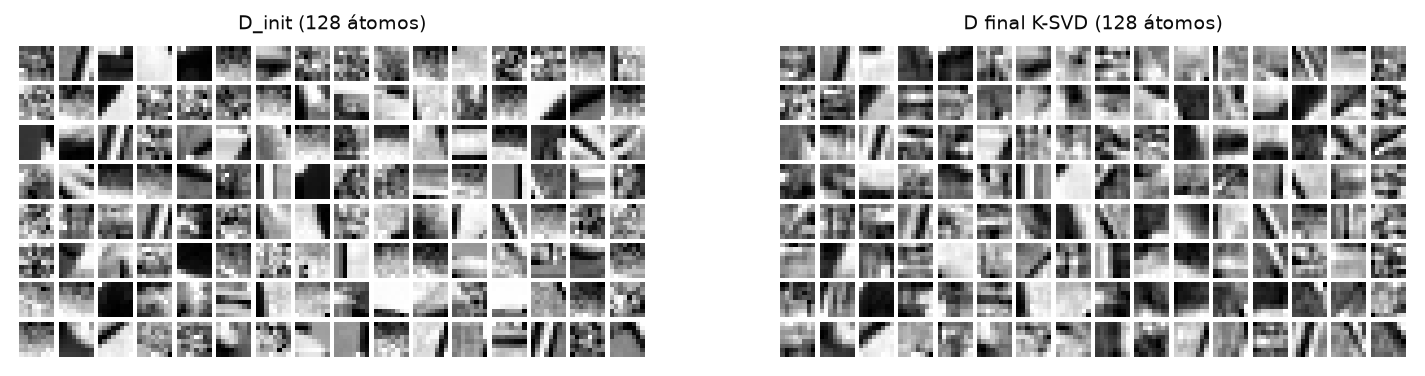
\includegraphics[width=0.95\linewidth]{../figuras/diccionarios.png}
\caption{Diccionario inicial (parches de entrenamiento) y diccionario final K-SVD.}\label{fig:dic}
\end{figure}

\section{Evaluación}
Se reconstruye coins limpia y ruidosa ($\sigma=20/255$, una realización con RNG 44, sin clipping; $\sigma$
empírica 0.07861). Para cada parche se codifica con OMP ($\le T_0$ átomos), se
restaura la media y se reensambla por promedio de solapamientos, sin clipping. Las métricas se calculan siempre
contra la imagen limpia. Verificación previa de métricas: imagen contra sí misma MSE $=0$, PSNR $=\infty$;
diferencia constante $0.1$: MSE $=0.0100$, PSNR
$=20.00$~dB. El tiempo es la mediana de 5
ejecuciones (extracción + OMP + reensamblado).

\begin{table}[h]\centering
\caption{Resultados sobre coins $128\times128$ (961 parches, K=128).}
\begin{tabular}{lrrrrr}\hline
entrada & $T_0$ & MSE & PSNR (dB) & coef. activos & tiempo (ms)\\\hline
ruidosa (sin procesar) & -- & 0.006179 & 22.09 & -- & -- \\
limpia & 2 & 0.002132 & 26.71 & 2.00 & 52.2 \\
limpia & 4 & 0.001264 & 28.98 & 4.00 & 88.5 \\
limpia & 8 & 0.000719 & 31.43 & 8.00 & 179.4 \\
ruidosa & 2 & 0.002784 & 25.55 & 2.00 & 51.9 \\
ruidosa & 4 & 0.002442 & 26.12 & 4.00 & 94.0 \\
ruidosa & 8 & 0.002730 & 25.64 & 8.00 & 168.1 \\
\hline\end{tabular}
\end{table}

\begin{figure}[h]\centering
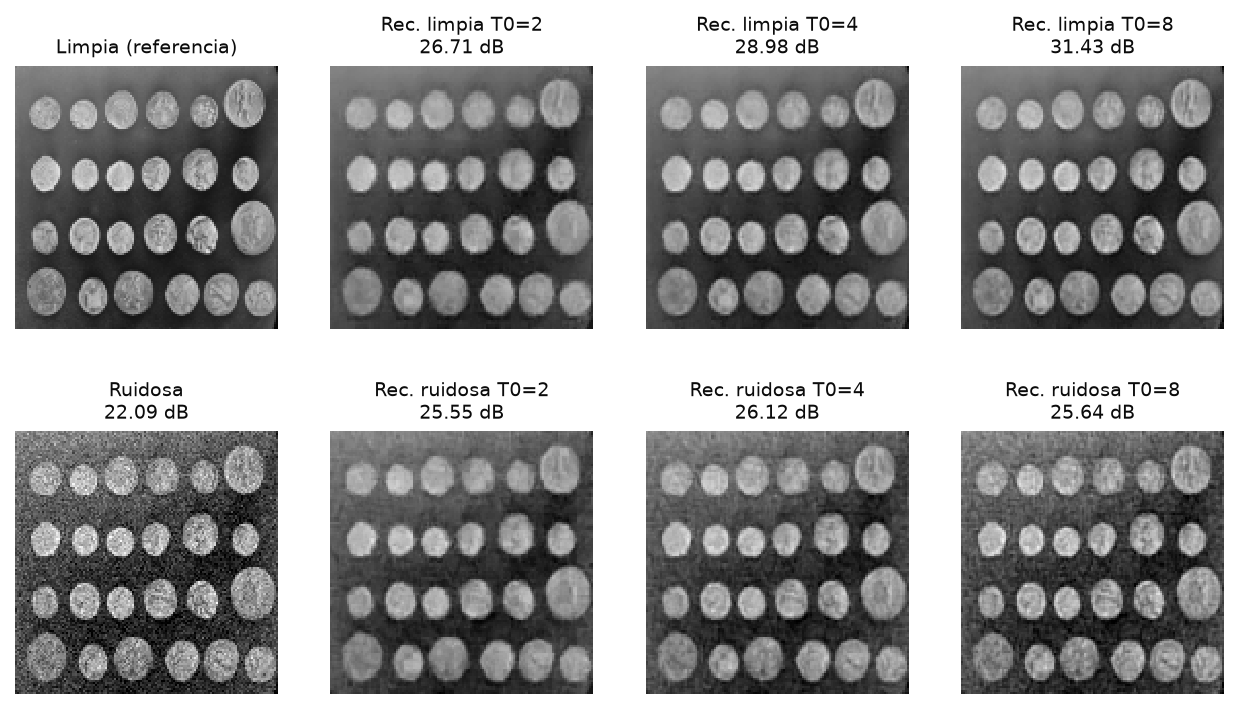
\includegraphics[width=\linewidth]{../figuras/reconstrucciones.png}
\caption{Reconstrucciones de la imagen limpia (arriba) y ruidosa (abajo) para cada $T_0$.}
\end{figure}

\begin{figure}[!ht]\centering
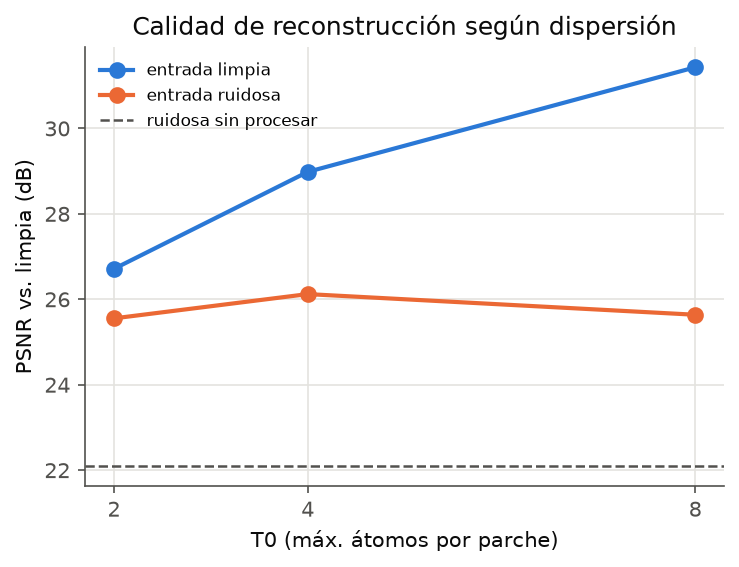
\includegraphics[width=0.55\linewidth]{../figuras/psnr_vs_t0.png}
\caption{PSNR frente a $T_0$. Línea discontinua: imagen ruidosa sin procesar.}
\end{figure}

\section{Discusión y conclusiones}
\begin{itemize}
\item Con la imagen limpia, el PSNR crece monótonamente con T0 (de 26.71 dB con T0=2 a 31.43 dB con T0=8): más átomos representan mejor la señal.
\item Con la imagen ruidosa el PSNR no es monótono: el máximo está en T0=4 (26.12 dB). Esto es consistente con un compromiso: con pocos átomos se pierde detalle y con muchos OMP también ajusta parte del ruido (interpretación, no medida directa).
\item Frente a la imagen ruidosa sin procesar (22.09 dB), la mejor reconstrucción mejora 4.03 dB. Es una ganancia real pero modesta; no se compara con el estado del arte.
\item La actividad dispersa media coincide exactamente con T0; el tiempo de reconstrucción crece con T0 y la codificación OMP ocupa en promedio el 88\% de ese tiempo.
\end{itemize}

\paragraph{Limitaciones.} Una sola imagen de entrenamiento y una de prueba, una realización de ruido, $T_0$
fijo en vez del criterio de error de \cite{elad2006}, sin promedio ponderado con la imagen ruidosa,
diccionario aprendido sobre parches limpios de otra imagen, coins redimensionada sin conservar su relación de
aspecto, y tiempos medidos en una sola máquina. Los resultados no son comparables directamente con las tablas
de los artículos.

\paragraph{Reproducibilidad.} \texttt{python run\_all.py} regenera todos los productos; \texttt{pytest}
verifica contratos y reproduce el pipeline en un directorio temporal. Versiones:\\
{\small\ttfamily python: 3.12.14\\
platform: Windows-11-10.0.26200-SP0\\
processor: Intel64 Family 6 Model 170 Stepping 4, GenuineIntel\\
numpy: 2.5.3\\
scipy: 1.18.1\\
scikit-learn: 1.9.1\\
scikit-image: 0.26.0\\
matplotlib: 3.11.2\\
pandas: 3.0.6\\
}

\begin{thebibliography}{9}
\bibitem{aharon2006} M. Aharon, M. Elad, A. Bruckstein. K-SVD: An Algorithm for Designing Overcomplete
Dictionaries for Sparse Representation. \emph{IEEE Trans. Signal Processing}, 54(11), 2006.
\url{https://doi.org/10.1109/TSP.2006.881199}
\bibitem{elad2006} M. Elad, M. Aharon. Image Denoising Via Sparse and Redundant Representations Over Learned
Dictionaries. \emph{IEEE Trans. Image Processing}, 15(12), 2006. \url{https://doi.org/10.1109/TIP.2006.881969}
\bibitem{sk} scikit-learn: \texttt{sklearn.linear\_model.orthogonal\_mp}; NumPy: \texttt{numpy.linalg.svd};
scikit-image: \texttt{skimage.data}, \texttt{skimage.metrics}.
\end{thebibliography}
\end{document}
